%\documentclass[12pt]{lettre}
%\usepackage[utf8]{inputenc}                
%\pagestyle{fancy}

%\title{Déclaration sur l'honneur de non-plagiat}   

%\begin{document}
%\maketitle	

\begin{center}
\LARGE
    Déclaration sur l'honneur de non-plagiat
\end{center}					 


\textbf{Je, soussigné,} 

\textbf{Nom, prénom :} CHIDA, Mohamed Omar 

\textbf{Élève ingénieur inscrit en 1ère année à TELECOM Nancy} 

\textbf{Numéro de carte étudiante :} 31730598 

\textbf{Année universitaire :} 2020 - 2021 

\textbf{Auteur, en collaboration avec DUMAS Mathis, TOUNSI OMEZZINE Chaima et ZHANG Céline, du rapport : } 

\begin{center}
\Large
    Algorithme pour l'analyse du SARS-COV2 
\end{center}


Je déclare sur l’honneur que ce rapport est le fruit d’un travail personnel et que je n’ai ni contrefait, ni falsifié, ni copié tout ou partie de l’œuvre d’autrui, en particulier, texte ou code informatique, afin de la faire passer pour mienne.

Je certifie donc que le travail rendu est un travail original et que les sources utilisées, notamment pour les formulations, les idées, les documentations, les raisonnements, les analyses, les schémas ou autres créations ont été mentionnées conformément aux usages en vigueur.

Je suis conscient que le fait de ne pas citer une source ou de ne pas la citer clairement et complètement est constitutif de plagiat, que le plagiat est considéré comme une faute grave au sein de l’Université et qu’il peut être sévèrement sanctionné. \\


\begin{flushright}
Fait à Nancy, le 03/01/2021 \\
Signature de l'étudiant:
\end{flushright}
\begin{figure}[!h]
    \begin{flushright}
        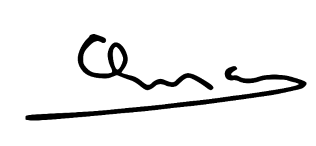
\includegraphics[scale=0.65]{Images/Intro/Signatures/omarr.png}
    \end{flushright}
\end{figure}

